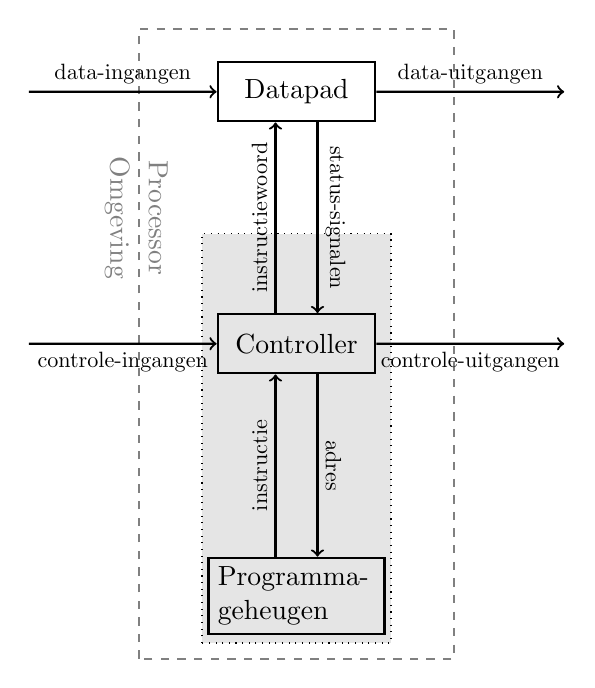
\begin{tikzpicture}[scale=0.8]
\draw[gray,dashed,thick] (-2.5,-7) rectangle (2.5,3);
\filldraw[fill=black!10!white,draw=black,dotted] (-1.5,-6.75) rectangle (1.5,-0.25);
\draw (-2.5,0) node[rotate=-90,gray,anchor=south]{Processor};
\draw (-2.5,0) node[rotate=-90,gray,anchor=north]{Omgeving};
\node[rectangle,thick,draw=black,minimum width=2 cm,minimum height=0.75 cm] (D) at (0,2) {Datapad};
\node[rectangle,thick,draw=black,minimum width=2 cm,minimum height=0.75 cm] (C) at (0,-2) {Controller};
\node[rectangle,thick,draw=black,minimum width=2 cm,text width=2 cm,minimum height=0.75 cm] (P) at (0,-6) {Programma\-geheugen};
\draw[->,thick] (D.south -| 0.3333,0) to node[midway,sloped,above,scale=0.8]{status-signalen} (C.north -| 0.3333,0);
\draw[->,thick] (C.north -| -0.3333,0) to node[midway,sloped,above,scale=0.8]{instructiewoord} (D.south -| -0.3333,0);
\draw[<-,thick] (C.west) to node[below,midway,scale=0.8]{controle-ingangen} (-4.25,-2);
\draw[->,thick] (C.east) to node[below,midway,scale=0.8]{controle-uitgangen} (4.25,-2);
\draw[<-,thick] (D.west) to node[above,midway,scale=0.8]{data-ingangen} (-4.25,2);
\draw[->,thick] (D.east) to node[above,midway,scale=0.8]{data-uitgangen} (4.25,2);
\draw[->,thick] (C.south -| 0.3333,0) to node[midway,sloped,above,scale=0.8]{adres} (P.north -| 0.3333,0);
\draw[->,thick] (P.north -| -0.3333,0) to node[midway,sloped,above,scale=0.8]{instructie} (C.south -| -0.3333,0);
\end{tikzpicture}